\documentclass{ximera}

\title{Linear Algebra}

\begin{document}
\begin{abstract}
The linear algebra portion of the self-evaluation test for the
University of Leuven's Masters of Artificial Intelligence program.
\end{abstract}
\maketitle

% Question 33
\begin{question}
True or false?  When the dot product of two vectors is negative, the angle between them is between 90 and 270 degrees.
\begin{solution}
\begin{multiple-choice}
\choice[correct]{true}
\choice{false}
\end{multiple-choice}
\end{solution}
Since the lengths of two vectors are always non-negative, a negative dot product indicates an angle with negative cosine. The range of angles with a negative cosine are those between 90 and 270 degrees.
\end{question}

% Question 34
\begin{question}
Given the vectors $u_1$ and $v_1$, give a matrix $M$ that transforms them
into $u_2$ and $v_2$; that is, find $M$ such that $M u_1=u_2$ and $M v_1=v_2$.

\begin{image}
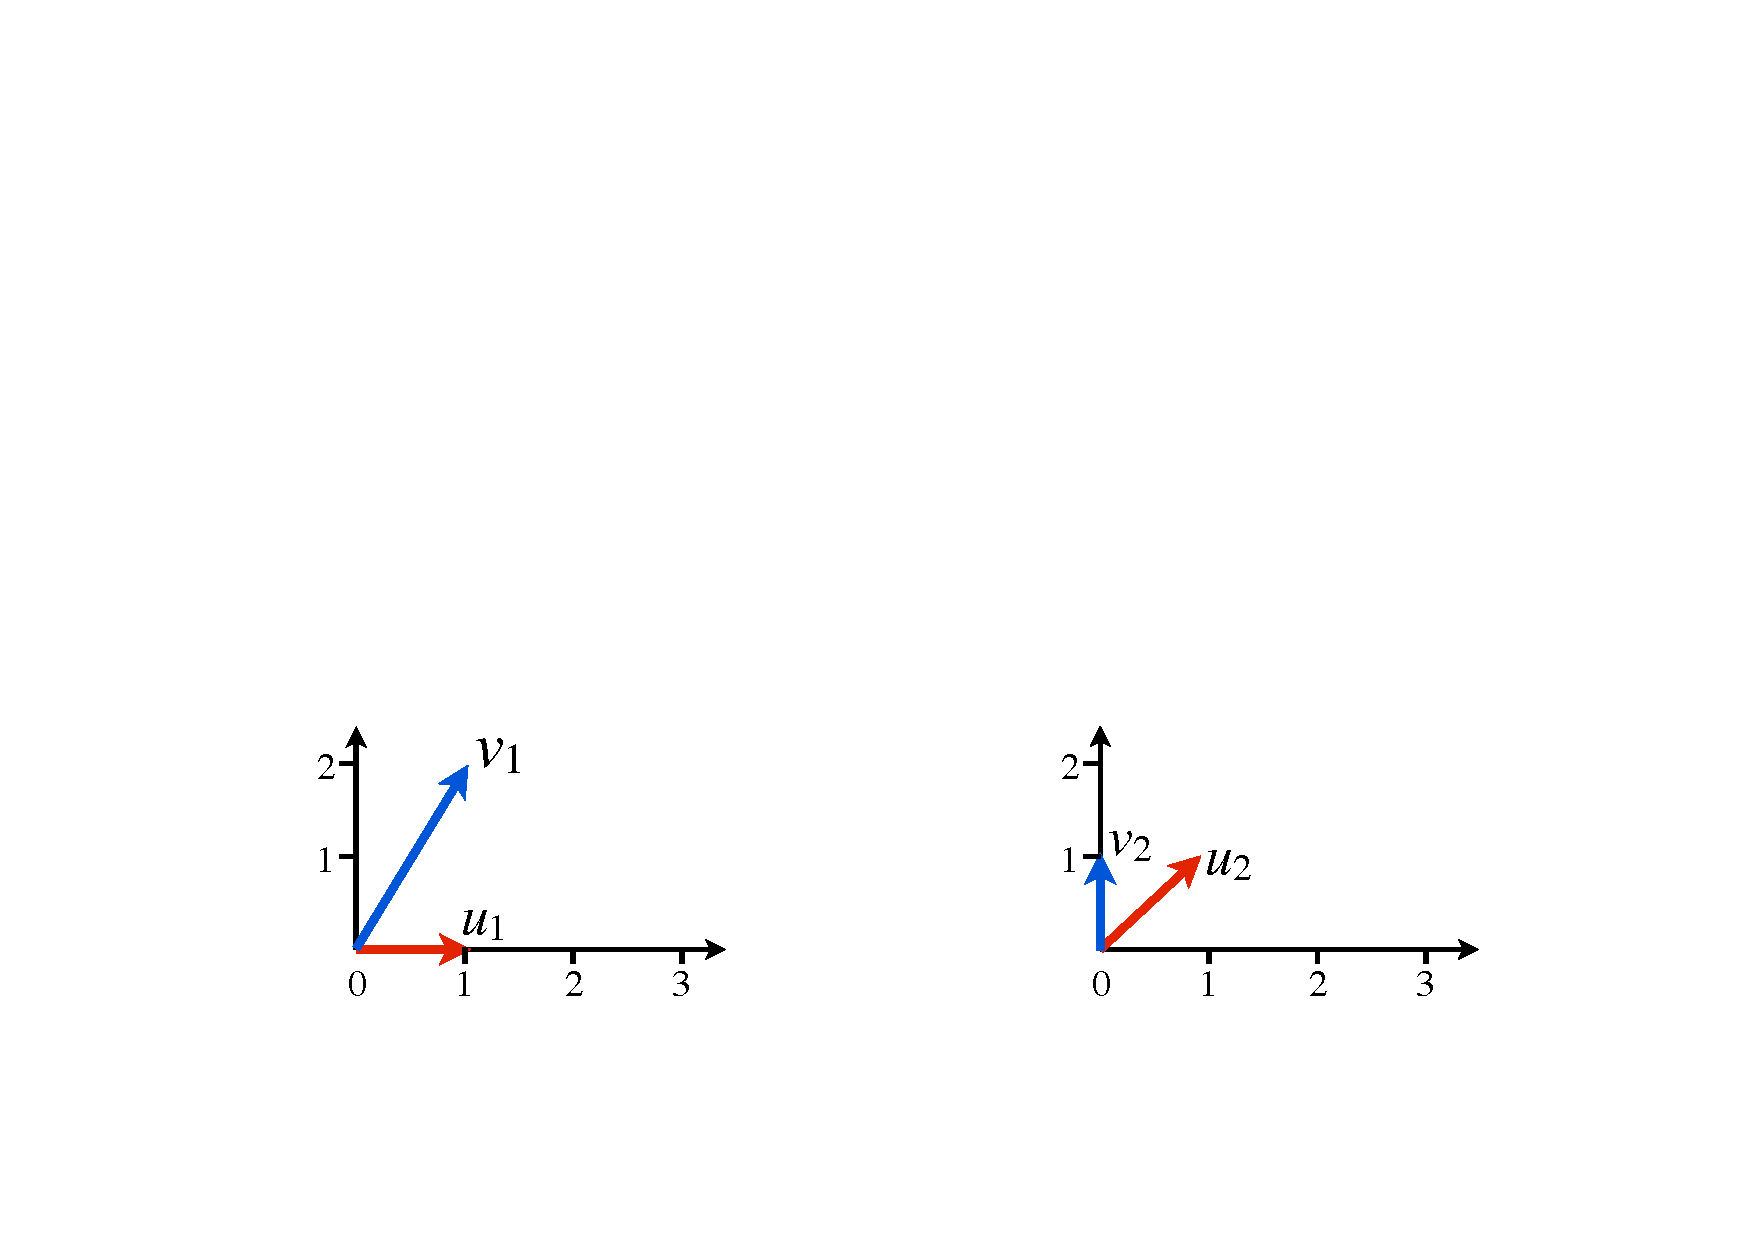
\includegraphics[width=0.6\textwidth]{fig.pdf}
\end{image}

\begin{solution}
\begin{matrix-answer}[name=M]
    correctMatrix = [['1','-1/2'],['1','0']]
\end{matrix-answer}
\end{solution}

Suppose that matrix $M$ contains these entries:
\begin{center}
\begin{equation*}
M =
\begin{bmatrix}
m_{11} & m_{12} \\
m_{21} & m_{22}
\end{bmatrix}
\end{equation*}
\end{center}

Since we have $M u_1 = u_2$:
\begin{align*}
&\begin{bmatrix}
m_{11} & m_{12} \\
m_{21} & m_{22}
\end{bmatrix}
\begin{bmatrix}
1 \\
0
\end{bmatrix}
= 
\begin{bmatrix}
1 \\
1
\end{bmatrix} \\
\\
& m_{11} = 1 \\
& m_{21} = 1
\end{align*}

Also from  $M v_1 = v_2$ we have:
\begin{align*}
&\begin{bmatrix}
m_{11} & m_{12} \\
m_{21} & m_{22}
\end{bmatrix}
\begin{bmatrix}
1 \\
2
\end{bmatrix}
= 
\begin{bmatrix}
0 \\
1
\end{bmatrix} \\
\\
& m_{11} + 2 m_{12} = 0 \\
& m_{21} + 2 m_{22} = 1 \\
\\
&m_{12} = - \frac{1}{2} \\
&m_{22} = 0
\end{align*}

So the transformation matrix is:
\begin{center}
\begin{equation*}
M =
\begin{bmatrix}
1 & -\frac{1}{2} \\
1 & 0
\end{bmatrix}
\end{equation*}
\end{center}


\end{question}

\end{document}
